\section{実際の OCaml ステッパ}
\label{section:ocaml stepper}

我々が実装した OCaml ステッパは、
\ref{section:try-with__stepper} 節で示した try-with と比べて
以下のような特徴がある。

\begin{itemize}
\item 型エラー等を想定しない。
\item 授業「関数型言語」で使用する構文のほぼ全てに対応している。
\item 関数適用が $\beta$ 簡約されるステップからその式が値になるステップまで飛ばす機能がある。
\end{itemize}

この節ではそれぞれについて述べる。

\subsection{型エラーについて}
\label{subsection:stepper__type}

OCaml ステッパでは、
まず入力プログラムを OCaml のパーザを利用して構文木にし、型チェックをする。
未定義変数エラーを含むシンタックスエラーや型エラーになった場合は
ステッパ本体のプログラムを起動せず、OCaml が示すエラーメッセージを表示する。
よって、コンパイルエラーがあるプログラムの構文木がステッパ関数に渡されることは無いという
仮定の上で実装されている。
ゼロ除算等の実行時エラーに関しては OCaml では例外の発生として処理されるので、
そのようにステップ実行処理を続行する。
ただし、例外が捕捉されないままその文の実行が終わってしまった場合はそこでステップ実行を終了する。

\subsection{対象構文}
\label{subsection:stepper__syntax}
% In Figure \ref{figure:ocamlstep},
% we show a reduction sequence produced by the actual stepping evaluator.
% 我々が実装した OCaml ステッパが出力するステップ列の例を図 \ref{figure:ocamlstep} に示す。
% The evaluator supports the following syntactic constructs:
このステッパは以下の構文に対応している。

\begin{itemize}
% \item integers, floating point numbers, booleans, characters, strings
% \item lists, tuples, records
% \item user-defined datatypes
% \item conditionals, let-expressions, recursive functions, pattern-matching
% \item exception handling operators
% \item printing functions and sequential execution
% \item the List module, user-defined modules
% \item references, arrays
\item 整数、実数、真偽値、文字、文字列型
\item リスト、組、レコード
\item ユーザ定義型
\item 条件分岐、変数定義、再帰関数定義、パターンマッチ
\item List モジュール、ユーザ定義モジュール
\item 例外処理
\item 標準出力関数、逐次実行
\item 書き換え可能な変数、配列
\end{itemize}

標準出力や書き換え可能な変数を含むプログラムでは、
標準出力された文字列や変数に格納された値などの「状態」をインタプリタが保持する必要がある。
状態の情報はステッパプログラム内の書き換え可能なグローバル変数の中に格納することで実装した。

\begin{figure}
  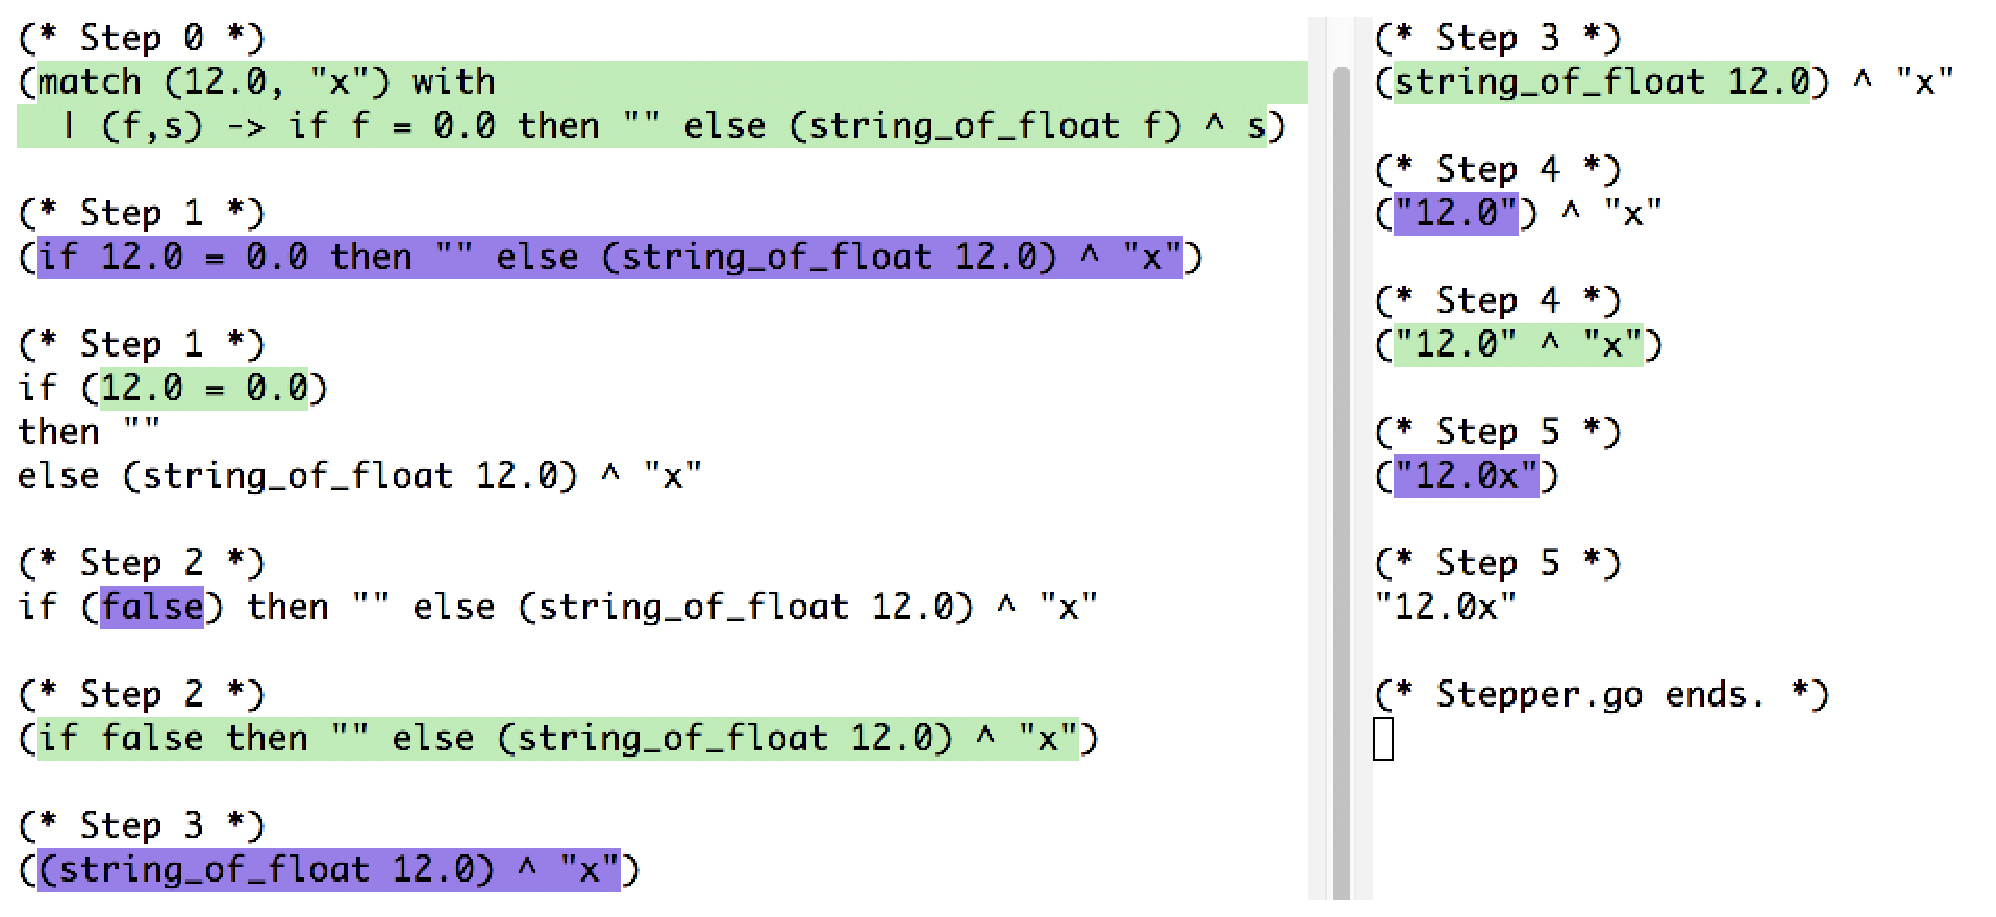
\includegraphics[width=14cm]{6/longexample.eps}
%   \caption{Evaluating programs using the actual stepper}
  \caption{実際のステッパでプログラムを実行する様子}
  \label{figure:ocamlstep}
\end{figure}

OCaml ステッパは他に授業で利用する一部の演算子などに対応している。
図 \ref{figure:ocamlstep} に実際のステップ列の例を示す。

% ref、配列を使うやつにする?

\subsection{関数適用のスキップ}
\label{subsection:skip}

\begin{figure}
  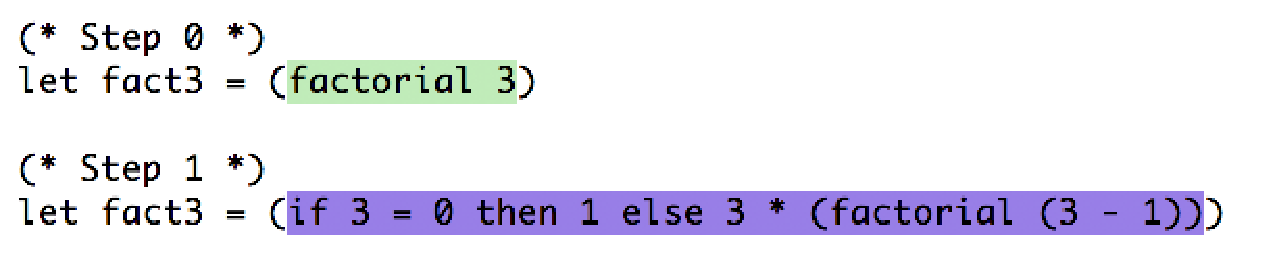
\includegraphics[width=10cm]{6/beforeskip.eps}
  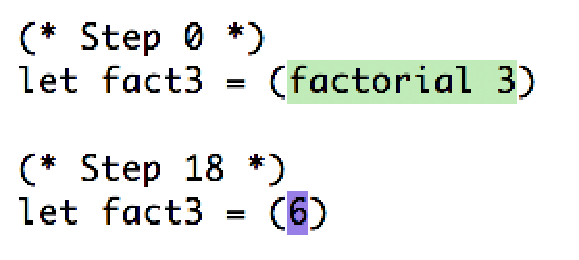
\includegraphics[width=4.3cm]{6/afterskip.eps}
%   \caption{Skipping evaluation of the factorial function}
  \caption{階乗関数をスキップする様子}
  \label{figure:factskip}
\end{figure}

% To allow the user to adjust granularity of steps,
% we provide an option for skipping
% the evaluation of the current function application.
プログラムのステップ数が多くなると、デバッグの目的でステップ実行をするときに
膨大な計算ステップを1つ1つ追って見るのは効率が悪く、
次第に実用に耐えるものではなくなってしまう。
そこで本研究では、「関数適用」を基準としてステップを飛ばす機能を追加した。

% Let us look at Figure \ref{figure:factskip},
% which shows skipping of the factorial function.
図 \ref{figure:factskip} に、階乗関数のスキップの様子を示す。
% By pressing the ``skip'' button,
% we can directly go from the program on the left to the one on the right,
% without seeing the intermediate steps that appear
% during the evaluation of the function's body.
左の状態で「skip」ボタンを押すと、関数の中身
\texttt{if 3 = 0 then 1 else 3 * (factorial (3 - 1))} が
\texttt{6} になるまでの実行ステップを見ることなく右の画面に移ることができる。
% This feature helps us focus on the steps we are interested in,
% allowing us to grasp the overall flow of the execution.
これによって見たいステップだけに注目することができ、実行の全体の流れを把握しやすくなる。

% The skipping feature requires some modifications to
% the \texttt{eval} function (Figure \ref{figure:skipapp}).
このスキップ機能は、
\ref{chapter:try-with} 章で try-with に対応したステッパ
(図 \ref{figure:stepper}) の eval 関数を
図 \ref{figure:skipapp} のように変更することで実装できる。
% The idea is to sandwich the steps within an application between two strings:
本研究では、飛ばすステップ列を
% \texttt{(* Application n start *)} and \texttt{(* Application n end *)}.
\texttt{(* Application n start *)} と \texttt{(* Application n end *)}
という 2 つの文字列で挟む方法をとった。
% Here, \texttt{n} tells us at which step we have entered the application.
\texttt{n} は関数適用の実行が始まるステップの番号である。
あるステップで実行が始まる関数適用は必ず 1 つ以下なので、
このステップ番号によって関数適用を一意に特定することができる。
% These strings are printed using the \texttt{apply\_start} and
% \texttt{apply\_end} functions,
% and help the Emacs Lisp program to hide unnecessary steps.
関数 \texttt{apply\_start :\ unit -> int} が前者を出力する関数、
関数 \texttt{apply\_end :\ int -> unit} が後者を出力する関数である。
表示処理をする Emacs Lisp プログラムがこれらの文字列を検索し、
間のステップを隠す処理をする。
% We show an example output sequence in Figure \ref{figure:skipping}.
スキップ機能を追加したステッパ関数の出力は例えば図 \ref{figure:skipping} のようになる。

\begin{figure}
\begin{alltt}
let rec eval expr ctxt = match expr with
    ...
  | App (e1, e2) ->
    begin
      let v2 = eval e2 (add ctxt (CAppR e1)) in
      let v1 = eval e1 (add ctxt (CAppL v2)) in
      match v1 with
      | Lam (x, e) ->
        let e' = subst e x v2 in
        \colorbox{lightgray}{let apply_num = apply_start () in}                (* output start mark *)
        memo (App (v1, v2)) e' ctxt;
        let v = eval e' ctxt in
        \colorbox{lightgray}{apply_end apply_num;}                               (* output end mark *)
        v
      | _ -> failwith "not a function"
    end
  | ...
\end{alltt}
\caption{関数適用をスキップするためのステッパ関数}
\label{figure:skipapp}
\end{figure}

\begin{figure}
\texttt{(* Step 0 *) (f 4) + \colorbox{lightgreen}{10 * 100}\\
(* Step 1 *) (f 4) + \colorbox{purple}{1000}\\
(* Application 1 start *)\\
(* Step 1 *) \colorbox{lightgreen}{f 4} + 1000\\
(* Step 2 *) \colorbox{purple}{(4 * 2) - 1} + 1000\\
(* Step 2 *) \colorbox{lightgreen}{(4 * 2} - 1) + 1000\\
(* Step 3 *) \colorbox{purple}{(8} - 1) + 1000\\
(* Step 3 *) \colorbox{lightgreen}{8 - 1} + 1000\\
(* Step 4 *) \colorbox{purple}{7} + 1000\\
(* Application 1 end *)\\
(* Step 4 *) \colorbox{lightgreen}{7 + 1000}\\
(* Step 5 *) \colorbox{purple}{1007}}
\caption{関数適用をスキップするためのステッパの出力}
\label{figure:skipping}
\end{figure}
